\documentclass[uplatex,dvipdfmx,11pt,notheorems]{beamer}
%%%% 和文用 %%%%%
\usepackage{bxdpx-beamer}
\usepackage{pxjahyper}
% \usepackage{minijs}%和文用
\renewcommand{\kanjifamilydefault}{\gtdefault}%和文用

%%%% スライドの見た目 %%%%%
\usetheme{Madrid}
\setbeamertemplate{frametitle}[default][center]
\setbeamertemplate{navigation symbols}{}
\setbeamercovered{transparent}%好みに応じてどうぞ)
\setbeamertemplate{footline}[page number]
\setbeamerfont{footline}{size=\normalsize,series=\bfseries}
\setbeamercolor{footline}{fg=black,bg=black}
\setbeamertemplate{footline}[frame number]
%%%%

%%%% 定義環境 %%%%%
\usepackage{amsmath,amssymb}
\usepackage{amsthm}
\theoremstyle{definition}
\newtheorem{theorem}{定理}
\newtheorem{definition}{定義}
\newtheorem{proposition}{命題}
\newtheorem{lemma}{補題}
\newtheorem{corollary}{系}
\newtheorem{conjecture}{予想}
\newtheorem*{remark}{Remark}
\renewcommand{\proofname}{}
%%%%%%%%%

%%%%% フォント基本設定 %%%%%
% \usepackage[T1]{fontenc}%8bit フォント
% \usepackage{textcomp}%欧文フォントの追加
% \usepackage[utf8]{inputenc}%文字コードをUTF-8
\usefonttheme{professionalfonts} %プロのフォント
\usepackage{color}
\usepackage{otf}%otfパッケージ
\usepackage{bm}%数式太字
%%%%%%%%%%
 
 \title[略タイトル]{輪講 - 第3回}%[略タイトル]{タイトル}
 \author[Xaro]{Ryosuke Horiuchi}%[略名前]{名前}
 \institute[JPN]{Tokyo, Japan}%[略所属]{所属}
 \date{\today}%日付
 \begin{document}

 \begin{frame}[plain]\frametitle{}
 \titlepage %表紙
 \end{frame}

 \begin{frame}\frametitle{Contents}
 \tableofcontents %目次
 \end{frame}

 \section{Gaussian distribution(ガウス分布)}
 %\subsection{ガウス分布の確率密度関数}
 \begin{frame}\frametitle{ガウス分布の確率密度関数}
 ガウス分布は正規分布とも言われ、平均$\mu$,分散$\sigma^{2}$を用いて、
 $$\mathcal{N}\left(x | \mu, \sigma^{2}\right)=\frac{1}{\left(2 \pi \sigma^{2}\right)^{1 / 2}} \exp \left\{-\frac{1}{2 \sigma^{2}}(x-\mu)^{2}\right\}$$
 と表せる.\\
 $\mathbf{x}$が$D$次元の場合には、平均$\boldsymbol{\mu}$,共分散$\mathbf{\Sigma}$を用いて
 $$\mathcal{N}(\mathbf{x} | \boldsymbol{\mu}, \mathbf{\Sigma})=\frac{1}{(2 \pi)^{D / 2}} \frac{1}{|\mathbf{\Sigma}|^{1 / 2}} \exp \left\{-\frac{1}{2}(\mathbf{x}-\boldsymbol{\mu})^{\mathrm{T}} \boldsymbol{\Sigma}^{-1}(\mathbf{x}-\boldsymbol{\mu})\right\}$$
 \end{frame}

\section{ガウス分布と最尤推定}
 \begin{frame}\frametitle{ガウス分布と最尤推定}
	$N$回の観測によって得られた観測値を$\mathbf{x}=\left(x_{1}, \dots, x_{N}\right)^{\mathrm{T}}$とする.
	ただし、これらはi.i.d (independent and identically distrubuted)と仮定.\\
	この時、その事象が起こる確率は、
	$$p\left(\mathbf{x} | \mu, \sigma^{2}\right)=\prod_{n=1}^{N} \mathcal{N}\left(x_{n} | \mu, \sigma^{2}\right)$$
	となる.\\

	しかし、実際、$\mu,\sigma^{2}$は未知 -- 最尤推定
	\begin{itemize}
		\item 最尤推定\\
		指数関数族に対しては、対数尤度を最大化することが多い.\\
		解析的に解きやすくなるだけでなく、数値計算の時もoverflowを起こしにくくなる.
	\end{itemize}
	
 \end{frame}

 \begin{frame}\frametitle{ガウス分布と最尤推定}
	$$\ln p\left(\mathbf{x} | \mu, \sigma^{2}\right)=-\frac{1}{2 \sigma^{2}} \sum_{n=1}^{N}\left(x_{n}-\mu\right)^{2}-\frac{N}{2} \ln \sigma^{2}-\frac{N}{2} \ln (2 \pi)$$
	これの$\mu,\sigma^{2}$による偏微分より、
	$$\mu_{\mathrm{ML}}=\frac{1}{N} \sum_{n=1}^{N} x_{n} = \text{標本平均}$$
	$$\sigma_{\mathrm{ML}}^{2}=\frac{1}{N} \sum_{n=1}^{N}\left(x_{n}-\mu_{\mathrm{ML}}\right)^{2} = \text{標本分散}$$
	となる.\\
\end{frame}

 \begin{frame}\frametitle{ガウス分布と最尤推定}
最尤推定でも求めた平均$\mu_{\mathrm{ML}}$と分散$\sigma_{\mathrm{ML}}^{2}$の期待値は、
$$\begin{aligned} \mathbb{E}\left[\mu_{\mathrm{ML}}\right] &=\mu \\ \mathbb{E}\left[\sigma_{\mathrm{ML}}^{2}\right] &=\left(\frac{N-1}{N}\right) \sigma^{2} \end{aligned}$$
\end{frame}

 \begin{frame}\frametitle{ガウス分布と最尤推定}
[証明]
	\begin{scriptsize}
	\begin{eqnarray}
	\mathbb{E}\left[\sigma_{\mathrm{ML}}^{2}\right] &=& \mathbb{E}\left[ \frac{1}{N} \sum_{n=1}^{N}\left(x_{n}-\frac{1}{N} \sum_{k=1}^{N} x_{k}\right)^{2} \right] \\
	&=&  \mathbb{E}\left[ \frac{1}{N} \sum_{n=1}^{N}\left(x_{n}^{2}-\frac{2}{N} x_{n} \sum_{k=1}^{N} x_{k} + \frac{1}{N^{2}} ( \sum_{k=1}^{N} x_{k} )^{2}\right) \right] \\
	&=&  \mathbb{E}\left[ \frac{1}{N} \sum_{n=1}^{N}x_{n}^{2} - \frac{1}{N^{2}} ( \sum_{k=1}^{N} x_{k} )^{2} \right] \\
	&=&  \mathbb{E}\left[ \frac{N-1}{N^{2}} \sum_{n=1}^{N}x_{n}^{2} - \frac{1}{N^{2}}  \sum_{i\neq j} x_{i}x_{j}  \right] \\
	&=&   \frac{N-1}{N^{2}} \sum_{n=1}^{N} \mathbb{E}\left[x_{n}^{2}\right] - \frac{1}{N^{2}}  \sum_{i\neq j}\mathbb{E}\left[ x_{i}x_{j}  \right] \\
	&=&   \frac{N-1}{N^{2}}  N (\sigma-\mu^{2}) - \frac{1}{N^{2}} N(N-1)(-\mu^{2}) \\
	&(\because& x_{i}: \text{i.i.d}, \text{for}  i=1,\dots, N) \\
	&=& \frac{N-1}{N} \sigma^{2} 
	\end{eqnarray}
	\end{scriptsize}
\end{frame}

\begin{frame}\frametitle{ガウス分布と最尤推定}
	e.g) 実際、図\ref{fig1}の時には、分散は平均しても正しいものとはならない.
	\begin{figure}[tb]
	\centering
	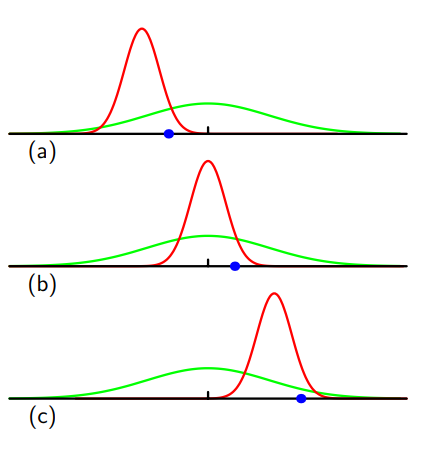
\includegraphics[width=4cm,clip]{gauss1.png}
	\caption{バイアスの発生}
	\label{fig1}
	\end{figure}
	つまり、平均はその平均を取ることで真の平均となるが、分散の平均は以前として小さく評価されてしまう. $N$が大きい時は問題ないがモデルが複雑になると注意しなければならない.
\end{frame}

\section{曲線フィッティング}
\begin{frame}\frametitle{曲線フィッティング}
	観測データが以下のように生成されているというモデルを立てる.
	$$p(t | x, \mathbf{w}, \beta)=\mathcal{N}\left(t | y(x, \mathbf{w}), \beta^{-1}\right)$$
	ただし、$\beta^{-1} = \sigma^{2}$とする. 
	\begin{figure}[tb]
	\centering
	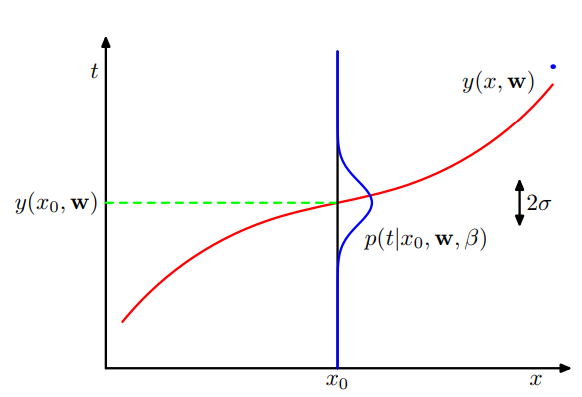
\includegraphics[width=6cm,clip]{gauss3.png}
	\caption{観測モデル}
	\label{fig1}
	\end{figure}
\end{frame}

\begin{frame}\frametitle{曲線フィッティングと最尤推定}
	訓練データ$\{\mathbf{x}, \mathbf{t}\}$から未知パラメータの$\mathbf{W},\beta$を最尤推定を用いて求める.
	$$p(\mathbf{t} | \mathbf{x}, \mathbf{w}, \beta)=\prod_{n=1}^{N} \mathcal{N}\left(t_{n} | y\left(x_{n}, \mathbf{w}\right), \beta^{-1}\right)$$
	対数尤度を取ると、
	$$\ln p(\mathbf{t} | \mathbf{x}, \mathbf{w}, \beta)=-\frac{\beta}{2} \sum_{n=1}^{N}\left\{y\left(x_{n}, \mathbf{w}\right)-t_{n}\right\}^{2}+\frac{N}{2} \ln \beta-\frac{N}{2} \ln (2 \pi)$$
	つまり、2乗和誤差を最小化することは、元のデータがあるガウス分布に従ってると仮定した上で対数最尤推定をすることと等価.
\end{frame}

\begin{frame}\frametitle{曲線フィッティングと最尤推定}

	最尤推定より求めた$\mathbf{w}_{\mathrm{ML}},\beta_{\mathrm{ML}}$を用いて、
	$$p\left(t | x, \mathbf{w}_{\mathrm{ML}}, \beta_{\mathrm{ML}}\right)=\mathcal{N}\left(t | y\left(x, \mathbf{w}_{\mathrm{ML}}\right), \beta_{\mathrm{ML}}^{-1}\right)$$
	とかける.ただし、
	$$\frac{1}{\beta_{\mathrm{ML}}}=\frac{1}{N} \sum_{n=1}^{N}\left\{y\left(x_{n}, \mathbf{w}_{\mathrm{ML}}\right)-t_{n}\right\}^{2}$$ 
\end{frame}

\begin{frame}\frametitle{曲線フィッティングとベイズ推定}
	\textcolor{red}{ベイズ理論を用いて最尤推定するとどうなるのだろうか.}\\
	事前分布を
	$$p(\mathbf{w} | \alpha)=\mathcal{N}\left(\mathbf{w} | \mathbf{0}, \alpha^{-1} \mathbf{I}\right)=\left(\frac{\alpha}{2 \pi}\right)^{(M+1) / 2} \exp \left\{-\frac{\alpha}{2} \mathbf{w}^{\mathrm{T}} \mathbf{w}\right\}$$
	とすると、ベイズの定理$p(\mathbf{w} | \mathbf{x}, \mathbf{t}, \alpha, \beta) \propto p(\mathbf{t} | \mathbf{x}, \mathbf{w}, \beta) p(\mathbf{w} | \alpha)$より、これに対して、対数尤度推定をすると
	$$\frac{\beta}{2} \sum_{n=1}^{N}\left\{y\left(x_{n}, \mathbf{w}\right)-t_{n}\right\}^{2}+\frac{\alpha}{2} \mathbf{w}^{\mathrm{T}} \mathbf{w}$$
	を最小化する問題と等価であることがわかる.これはMAP(maximum posterior)と呼ばれる.\\
	上式は、正則化された2乗和誤差関数と等価であることもわかる.
\end{frame}

\section{ベイズ曲線フィッティング}
\begin{frame}\frametitle{ベイズ曲線フィッティング}
	$p(\mathbf{w} | \mathbf{x}, \mathbf{t}, \alpha, \beta)$ではなく、$p(t | x, \mathbf{x}, \mathbf{t})$がわかって初めて、予測ができる.$\alpha, \beta$を省略して、
	$$p(t | x, \mathbf{x}, \mathbf{t})=\int p(t | x, \mathbf{w}) p(\mathbf{w} | \mathbf{x}, \mathbf{t}) \mathrm{d} \mathbf{w}$$
	とかける. \textcolor{green}{ガウス分布のすばらしい性質(興味のある人は2.3~へ)}によって、これらは解析的に計算することができて、
	$p(t | x, \mathbf{x}, \mathbf{t})=\mathcal{N}\left(t | m(x), s^{2}(x)\right)$とすると、
	$$\begin{aligned} m(x) &=\beta \phi(x)^{\mathrm{T}} \mathbf{S} \sum_{n=1}^{N} \phi\left(x_{n}\right) t_{n} \\ s^{2}(x) &=\beta^{-1}+\textcolor{red}{\phi(x)^{\mathrm{T}} \mathbf{S} \phi(x)} \end{aligned}$$
	ただし、$\phi_{i}(x)=x^{i} \text { for } i=0, \dots, M$として、
	$$\mathbf{S}^{-1}=\alpha \mathbf{I}+\beta \sum_{n=1}^{N} \phi\left(x_{n}\right) \phi(x)^{\mathrm{T}}$$


\end{frame}

\begin{frame}\frametitle{ベイズ曲線フィッティング}
分散に注目すると赤字の部分がベイズ的な扱いによって、生じた部分.

\begin{figure}[tb]
	\centering
	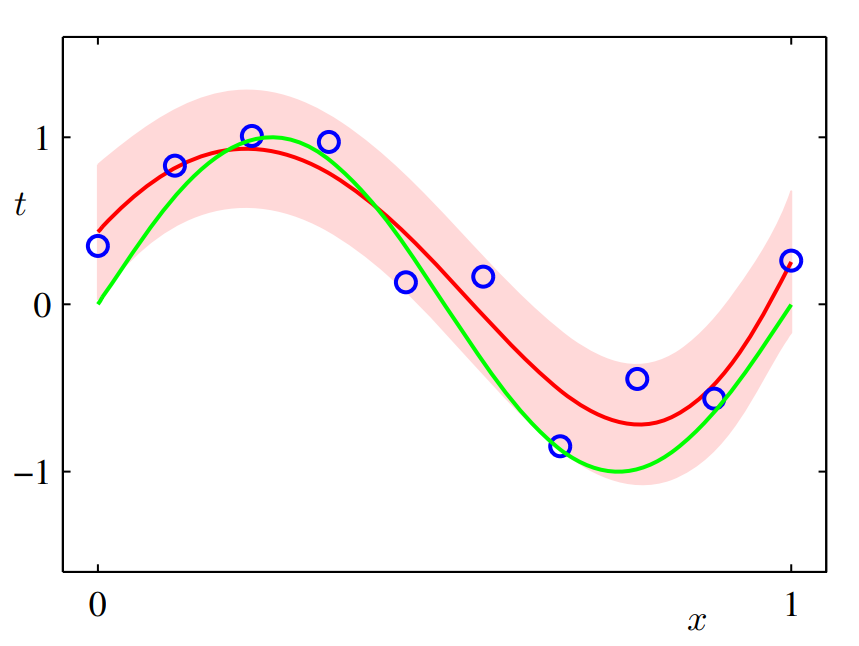
\includegraphics[width=6cm,clip]{gauss4.png}
	\caption{$M=9$の場合における比較. 赤線:ベイズ、緑:普通の最尤推定}
	\label{fig1}
	\end{figure}



\end{frame}



 \begin{frame}\frametitle{Contents}
 \tableofcontents %目次
 \end{frame}
\end{document}
